\section{What Was Held Fixed, and What Was Checked}
\label{app:realized}
The supporting analyses address four questions: whether the intended allocations were achieved, whether the estimates have adequate patient support, whether recovery depends on the assignment, and whether calibration or partition variation changes the interpretation. Repeated execution records are summarized as ranges; paired uncertainty intervals are retained for the primary damage and weighting comparisons. Ranges describe observed variation, not confidence intervals.

\subsection{Allocation and patient coverage}
\label{app:realized-construction}
Table~\ref{tab:realized-support} separates class imbalance from patient coverage. Within each partition, balanced and balanced-spread training use identical class-specific patch counts. Their patient counts differ substantially, especially on TCGA-UT. Moderate and severe allocations meet their target ratios of 9--11 and 90--110, respectively; none is off-target or collapses to balance. Small departures from a ratio of one in balanced training reflect integer allocation.

\begin{table}[H]
\centering\footnotesize\setlength{\tabcolsep}{3pt}
% Generated by assets/build_readable_appendix.mjs; do not edit.
\begin{tabular}{@{}lrrrr@{}}
\toprule
Allocation & Patients & Patches & $\rho$ & $1-H_{\rm norm}$ \\
\midrule
\multicolumn{5}{@{}l}{\textbf{BRACS}} \\
Natural & \num{103} & \num{193010} to \num{217704} & \num{5.722} to \num{8.297} & \num{0.1178} to \num{0.1432} \\
Balanced & \num{78} to \num{89} & \num{13982} to \num{27202} & \num{1.000} to \num{1.001} & \num{0.0000} \\
Balanced spread & \num{103} & \num{13982} to \num{27202} & \num{1.000} to \num{1.001} & \num{0.0000} \\
Moderate & \num{78} to \num{89} & \num{13982} to \num{27202} & \num{10.003} to \num{10.007} & \num{0.1280} \\
Severe & \num{78} to \num{89} & \num{13982} to \num{27202} & \num{100.301} to \num{100.467} & \num{0.3530} \\
Severe spread & \num{103} & \num{13982} to \num{27202} & \num{100.301} to \num{100.467} & \num{0.3530} \\
\multicolumn{5}{@{}l}{\textbf{TCGA-UT}} \\
Natural & \num{4983} & \num{1116020} to \num{1121580} & \num{17.850} to \num{18.395} & \num{0.0754} to \num{0.0765} \\
Balanced & \num{671} to \num{917} & \num{36988} to \num{52204} & \num{1.001} & \num{0.0000} \\
Balanced spread & \num{4983} & \num{36988} to \num{52204} & \num{1.001} & \num{0.0000} \\
Moderate & \num{671} to \num{917} & \num{36988} to \num{52204} & \num{9.992} to \num{10.003} & \num{0.0609} \\
Severe & \num{671} to \num{917} & \num{36988} to \num{52204} & \num{90.107} to \num{100.500} & \num{0.1735} to \num{0.1792} \\
Severe spread & \num{4203} to \num{4983} & \num{36988} to \num{52204} & \num{90.107} to \num{100.500} & \num{0.1735} to \num{0.1792} \\
\bottomrule
\end{tabular}

\caption{Allocation ranges across the three partitions and available assignments. Patients are unique contributing patients, not summed class counts. Patch counts refer to one realized training allocation. Spread increases patient coverage at matched patch counts; it does not necessarily reach every eligible patient under severe allocation.}
\label{tab:realized-support}
\end{table}

\noindent For BRACS, balanced training uses \num{13982}--\num{27202} patches from \num{78}--\num{89} patients, compared with \num{103} patients under balanced spread. The corresponding TCGA-UT comparison uses \num{36988}--\num{52204} patches from \num{671}--\num{917} versus \num{4983} patients. The patient inventory is therefore exhausted by balanced spread on both datasets, while TCGA-UT severe spread reaches \num{4203}--\num{4983} patients.

\subsection{Patient support and complete comparisons}
\label{app:realized-validity}
The \emph{bootstrap patient-support check} evaluates the planned resampling before training, using only patient identifiers, partition membership, and class labels. It checks whether each pooled class has at least five contributing patients, whether the \num{2.5}th percentile of its Kish effective count is at least five, and whether a single patient carries more than half the weight in at most \num{5}\% of replicates. Failure would restrict the dataset to descriptive estimates.

Both datasets pass. The closest effective-count margins are \num{5.5} for ductal carcinoma in situ on BRACS and \num{6.6} for uterine carcinosarcoma on TCGA-UT. No pooled class has a dominant patient in any replicate.

The qualification changes at the individual partition level. BRACS flags atypical ductal hyperplasia, ductal carcinoma in situ, and flat epithelial atypia. TCGA-UT flags adrenocortical carcinoma, kidney chromophobe, mesothelioma, ovarian serous cystadenocarcinoma, pheochromocytoma and paraganglioma, rectum adenocarcinoma, thymoma, uterine carcinosarcoma, and uveal melanoma. Class-specific estimates from those partitions need caution; the confirmatory comparisons use the valid pooled patient support.

All five confirmation seeds and all three partitions are present in every required block, yielding \num{378} planned comparisons per dataset. Relative achieved-severity spread is at most \num{0.002} on BRACS and \num{0.010} on TCGA-UT, below the \num{0.5} limit. Semantic-scale weighting records zero invalid draws across \num{195} reweighting pools per dataset: its fallback to unit weights never occurs.

\subsection{What tuning selected}
\label{app:realized-deviations}
Training budgets count example presentations, not optimizer updates: controlled and natural budgets are \num{503880} and \num{6521970} on BRACS, and \num{1343760} and \num{33480600} on TCGA-UT. A method consuming $e_m$ examples per update receives $\lceil E/e_m\rceil$ updates, with checkpoint spacing adjusted to keep approximately the same number of validation passes.

Tables~\ref{tab:tuning-selections} and~\ref{tab:tuning-tcga} show which parameter values were selected and how often the strength was zero. They summarize the \num{392} recorded condition--assignment--method entries, including configurations reused across assignments; these are not \num{392} independent tuning exercises. No entry selects a learning rate at the boundary of the candidate range. This rules out observed boundary selections, but does not establish that a wider range could not improve validation performance.

\begin{table}[H]
\centering\small
\input{assets/readable/tuning_BRACS.tex}
\caption{BRACS tuning summary. Ranges span recorded selections; zero-strength counts use entries with a strength parameter as denominator. Strength has a method-specific meaning and cannot be compared numerically across methods.}
\label{tab:tuning-selections}
\end{table}
\begin{table}[H]
\centering\small
% Generated by assets/build_readable_appendix.mjs; do not edit.
\begin{tabular}{@{}p{4.1cm}rrr@{}}
\toprule
Method & Learning rate & Strength & Zero strength \\
\midrule
Balanced sampling & \num{0.00003} to \num{0.00010} & \num{0.0000} to \num{1.0000} & 3/13 \\
CE & \num{0.00010} to \num{0.00030} & --- & --- \\
CE + soft $F_1$ & \num{0.00003} to \num{0.00010} & \num{1.0000} to \num{16.0000} & 0/13 \\
CE + soft MCC & \num{0.00003} to \num{0.00010} & \num{1.0000} to \num{16.0000} & 0/13 \\
CFAL & \num{0.00010} to \num{0.00030} & \num{0.2500} to \num{4.0000} & 0/13 \\
Nominal support & \num{0.00003} to \num{0.00010} & \num{0.9900} to \num{0.9999} & 0/13 \\
cRT & \num{0.00100} to \num{0.00300} & --- & --- \\
Focal loss & \num{0.00003} to \num{0.00010} & \num{0.0000} & 13/13 \\
Independent support & \num{0.00010} to \num{0.00030} & \num{0.8000} to \num{0.9990} & 0/13 \\
Logit adjustment (train) & \num{0.00010} & \num{0.5000} to \num{2.0000} & 0/13 \\
OKO & \num{0.00030} to \num{0.00100} & \num{1.0000} to \num{4.0000} & 0/13 \\
Difficulty & \num{0.00010} to \num{0.00030} & \num{0.2500} & 0/13 \\
Logit adjustment (post-hoc) & Reused CE & \num{0.2500} to \num{1.0000} & 0/13 \\
Diversity & \num{0.00010} to \num{0.00030} & \num{0.2500} to \num{1.0000} & 0/13 \\
Prevalence & \num{0.00003} to \num{0.00010} & \num{0.0000} to \num{1.0000} & 3/13 \\
\bottomrule
\end{tabular}

\caption{TCGA-UT tuning summary, using the same conventions as Table~\ref{tab:tuning-selections}. Post-hoc logit adjustment reuses the cross-entropy checkpoint.}
\label{tab:tuning-tcga}
\end{table}

\noindent Zero strength does not always mean ordinary cross-entropy. The soft-$F_1$ and soft-MCC hybrids retain balanced sampling; focal loss at $\gamma=0$ retains class-aware $\alpha$. These selected candidates were trained with those mechanisms intact. Most methods receive \num{16} candidates, cross-entropy and classifier retraining four, and post-hoc logit adjustment one shard without new training.

Selection maximizes natural-prevalence validation balanced accuracy, with macro $F_1$ and negative log likelihood as successive tie-breakers. It pools assignments and does not optimize the tail-group probability-quality endpoint. Consequently, weak recovery can reflect both the signal and the selected operating point; a calibration deterioration describes a method tuned for discrimination.

Two protocol deviations were fixed before definitive results were read. Materiality thresholds use the pilot-defined quantities $\max(1,2\sigma_{\rm seed})$ for discrimination and $2\sigma_{\rm seed}$ for calibration: \num{1.443} percentage points and \num{0.14782} nats on BRACS, versus \num{1.000} point and \num{0.06095} nats on TCGA-UT. The defining estimator is patient-macro rather than patch-micro and pools each patient's partition appearances, matching the crossed patient bootstrap.

\clearpage
\section{How Large Was the Damage?}
\label{app:damage-estimates}
The natural condition provides context but is not the reference for these deficits. Moderate and severe concentrated training are compared with concentrated balanced training; severe spread and patient shortage use balanced spread. Positive values mean worse performance under deprivation. Tables~\ref{tab:discrimination-deficit} and~\ref{tab:calibration-deficit} preserve every assignment and its paired interval, making the distinction between an imprecise deficit and a sub-threshold one explicit.

\begin{table}[H]
\centering\small\setlength{\tabcolsep}{4pt}
% Generated by assets/build_readable_appendix.mjs; do not edit.
\begin{tabular}{@{}lllrl@{}}
\toprule
Dataset & Comparison & Assignment & Deficit [95\% CI] & Eligible \\
\midrule
BRACS & Patient shortage & Native & 2.91 [1.02, 5.19] & Yes \\
BRACS & Patient shortage & Aligned & 3.03 [1.02, 5.31] & Yes \\
BRACS & Patient shortage & Reversed & 2.62 [0.53, 5.02] & Yes \\
BRACS & Moderate & Native & 3.34 [1.72, 5.09] & Yes \\
BRACS & Moderate & Aligned & 1.50 [-0.40, 3.39] & Imprecise \\
BRACS & Moderate & Reversed & 8.17 [6.09, 10.60] & Yes \\
BRACS & Severe & Native & 5.45 [3.27, 7.81] & Yes \\
BRACS & Severe & Aligned & 4.30 [2.08, 6.59] & Yes \\
BRACS & Severe & Reversed & 13.23 [10.78, 15.84] & Yes \\
BRACS & Severe spread & Native & 8.43 [5.79, 11.37] & Yes \\
BRACS & Severe spread & Aligned & 4.15 [1.97, 6.62] & Yes \\
BRACS & Severe spread & Reversed & 13.77 [11.33, 16.34] & Yes \\
TCGA-UT & Patient shortage & Native & 4.76 [4.13, 5.41] & Yes \\
TCGA-UT & Patient shortage & Aligned & 4.83 [4.21, 5.46] & Yes \\
TCGA-UT & Patient shortage & Reversed & 4.83 [4.22, 5.45] & Yes \\
TCGA-UT & Moderate & Native & 0.36 [0.12, 0.61] & Below minimum \\
TCGA-UT & Moderate & Aligned & 0.13 [-0.13, 0.40] & Below minimum \\
TCGA-UT & Moderate & Reversed & 0.45 [0.17, 0.72] & Below minimum \\
TCGA-UT & Severe & Native & 1.79 [1.36, 2.23] & Yes \\
TCGA-UT & Severe & Aligned & 1.33 [0.86, 1.79] & Yes \\
TCGA-UT & Severe & Reversed & 1.45 [0.97, 1.93] & Yes \\
TCGA-UT & Severe spread & Native & 4.96 [4.30, 5.65] & Yes \\
TCGA-UT & Severe spread & Aligned & 3.07 [2.62, 3.52] & Yes \\
TCGA-UT & Severe spread & Reversed & 2.40 [1.94, 2.88] & Yes \\
\bottomrule
\end{tabular}

\caption{Balanced-accuracy loss in percentage points, with paired 95\% intervals. Eligibility requires both the dataset's minimum deficit and an interval excluding zero. TCGA-UT moderate has small positive estimates, not an established absence of loss.}
\label{tab:discrimination-deficit}
\end{table}

\begin{table}[H]
\centering\small\setlength{\tabcolsep}{4pt}
% Generated by assets/build_readable_appendix.mjs; do not edit.
\begin{tabular}{@{}lllrl@{}}
\toprule
Dataset & Comparison & Assignment & Deficit [95\% CI] & Eligible \\
\midrule
BRACS & Patient shortage & Native & 0.138 [0.064, 0.216] & Below minimum \\
BRACS & Patient shortage & Aligned & 0.140 [0.071, 0.213] & Below minimum \\
BRACS & Patient shortage & Reversed & 0.134 [0.061, 0.209] & Below minimum \\
BRACS & Moderate & Native & 0.186 [-0.007, 0.397] & Imprecise \\
BRACS & Moderate & Aligned & 0.379 [0.157, 0.715] & Yes \\
BRACS & Moderate & Reversed & 0.754 [0.180, 1.706] & Yes \\
BRACS & Severe & Native & 0.688 [0.332, 1.099] & Yes \\
BRACS & Severe & Aligned & 0.729 [0.488, 1.045] & Yes \\
BRACS & Severe & Reversed & 1.744 [1.208, 2.295] & Yes \\
BRACS & Severe spread & Native & 0.205 [0.100, 0.334] & Yes \\
BRACS & Severe spread & Aligned & 0.908 [0.575, 1.267] & Yes \\
BRACS & Severe spread & Reversed & 1.129 [0.830, 1.474] & Yes \\
TCGA-UT & Patient shortage & Native & 0.263 [0.226, 0.304] & Yes \\
TCGA-UT & Patient shortage & Aligned & 0.259 [0.224, 0.296] & Yes \\
TCGA-UT & Patient shortage & Reversed & 0.258 [0.224, 0.295] & Yes \\
TCGA-UT & Moderate & Native & -0.199 [-0.244, -0.152] & Below minimum \\
TCGA-UT & Moderate & Aligned & -0.118 [-0.153, -0.084] & Below minimum \\
TCGA-UT & Moderate & Reversed & -0.062 [-0.093, -0.038] & Below minimum \\
TCGA-UT & Severe & Native & -0.168 [-0.226, -0.100] & Below minimum \\
TCGA-UT & Severe & Aligned & 0.143 [0.081, 0.219] & Yes \\
TCGA-UT & Severe & Reversed & -0.031 [-0.076, 0.020] & Below minimum \\
TCGA-UT & Severe spread & Native & 0.193 [0.139, 0.263] & Yes \\
TCGA-UT & Severe spread & Aligned & 0.199 [0.151, 0.256] & Yes \\
TCGA-UT & Severe spread & Reversed & 0.081 [0.042, 0.121] & Yes \\
\bottomrule
\end{tabular}

\caption{Tail-group negative-log-likelihood increase in nats, with paired 95\% intervals. Negative values mean improved probability quality. TCGA-UT moderate improves this endpoint under all three assignments, even though balanced accuracy falls slightly.}
\label{tab:calibration-deficit}
\end{table}

\noindent This contrast matters for interpretation: moderate deprivation on TCGA-UT is not simply too noisy to detect. Native and reversed balanced-accuracy intervals exclude zero, but their estimates remain below the one-point minimum. All three probability-quality intervals instead favour moderate training. Neither finding makes the much larger natural training set an appropriate causal reference.

\clearpage
\section{Which Signals Recover the Loss?}
\label{app:recovery-estimates}
The main-text recovery map shows the pattern; the following tables retain the uncertainty behind it. Each cell gives recovery as a percentage, its paired bootstrap 95\% interval, and the Holm-adjusted permutation $p$-value. Zero means no repair and 100\% means the balanced reference is reached. Negative recovery means further damage. Only eligible comparisons appear; absent rows must not be interpreted as zero recovery. Nominal and independent denote the corresponding support-weighted cross-entropy methods.

\begin{table}[H]
\centering\footnotesize\setlength{\tabcolsep}{3pt}\renewcommand{\arraystretch}{1.35}
% Generated by assets/build_readable_appendix.mjs; do not edit.
\begin{tabular}{@{}lccccc@{}}
\toprule
Comparison & Prevalence & Nominal & Independent & Difficulty & Diversity \\
\midrule
\shortstack[l]{Moderate\\Native} & \shortstack{81.5\\{}[41.9, 123.7]\\$p=0.0130$} & \shortstack{89.2\\{}[54.9, 130.7]\\$p=0.0022$} & \shortstack{19.7\\{}[-19.0, 55.7]\\$p=1.0000$} & \shortstack{12.1\\{}[-26.3, 45.3]\\$p=1.0000$} & \shortstack{14.2\\{}[-41.5, 62.2]\\$p=1.0000$} \\
\shortstack[l]{Moderate\\Reversed} & \shortstack{84.0\\{}[72.0, 96.2]\\$p=0.0026$} & \shortstack{83.3\\{}[69.6, 96.9]\\$p=0.0011$} & \shortstack{5.1\\{}[-14.4, 20.2]\\$p=1.0000$} & \shortstack{-7.8\\{}[-24.4, 5.9]\\$p=1.0000$} & \shortstack{-6.4\\{}[-27.9, 12.6]\\$p=1.0000$} \\
\shortstack[l]{Severe\\Native} & \shortstack{76.8\\{}[44.1, 103.0]\\$p=0.1214$} & \shortstack{63.7\\{}[35.3, 88.0]\\$p=0.1297$} & \shortstack{10.6\\{}[-14.9, 32.3]\\$p=1.0000$} & \shortstack{-27.3\\{}[-63.7, -7.0]\\$p=0.0603$} & \shortstack{-16.5\\{}[-54.8, 4.9]\\$p=1.0000$} \\
\shortstack[l]{Severe\\Aligned} & \shortstack{65.4\\{}[33.0, 106.1]\\$p=0.3344$} & \shortstack{42.6\\{}[0.2, 76.7]\\$p=1.0000$} & \shortstack{2.4\\{}[-19.3, 21.4]\\$p=1.0000$} & \shortstack{16.4\\{}[-7.1, 43.7]\\$p=1.0000$} & \shortstack{-5.9\\{}[-52.4, 23.7]\\$p=1.0000$} \\
\shortstack[l]{Severe\\Reversed} & \shortstack{79.4\\{}[69.1, 88.9]\\$p=0.0006$} & \shortstack{73.6\\{}[61.9, 85.6]\\$p=0.0006$} & \shortstack{11.1\\{}[4.6, 18.4]\\$p=0.0505$} & \shortstack{-5.9\\{}[-12.0, 0.2]\\$p=0.8122$} & \shortstack{-1.0\\{}[-9.2, 6.4]\\$p=1.0000$} \\
\shortstack[l]{Severe spread\\Native} & \shortstack{87.1\\{}[70.9, 105.8]\\$p=0.0016$} & \shortstack{83.1\\{}[67.5, 101.3]\\$p=0.0006$} & \shortstack{11.1\\{}[-3.3, 22.7]\\$p=1.0000$} & \shortstack{2.1\\{}[-17.3, 19.0]\\$p=1.0000$} & \shortstack{-2.6\\{}[-15.1, 7.4]\\$p=1.0000$} \\
\shortstack[l]{Severe spread\\Aligned} & \shortstack{46.6\\{}[0.5, 82.3]\\$p=1.0000$} & \shortstack{45.5\\{}[8.5, 75.5]\\$p=1.0000$} & \shortstack{-13.5\\{}[-46.1, 5.9]\\$p=1.0000$} & \shortstack{-14.5\\{}[-83.6, 20.4]\\$p=1.0000$} & \shortstack{-14.5\\{}[-61.6, 11.2]\\$p=1.0000$} \\
\shortstack[l]{Severe spread\\Reversed} & \shortstack{82.4\\{}[71.4, 94.0]\\$p=0.0006$} & \shortstack{79.1\\{}[68.5, 90.6]\\$p=0.0006$} & \shortstack{5.1\\{}[-0.6, 11.3]\\$p=0.8772$} & \shortstack{-0.8\\{}[-9.1, 5.9]\\$p=1.0000$} & \shortstack{3.0\\{}[-3.7, 9.2]\\$p=1.0000$} \\
\shortstack[l]{Patient shortage\\Native} & \shortstack{0.3\\{}[-1.4, 3.1]\\$p=1.0000$} & \shortstack{0.5\\{}[-1.3, 3.3]\\$p=1.0000$} & \shortstack{1.3\\{}[-0.8, 5.5]\\$p=1.0000$} & \shortstack{-5.8\\{}[-25.6, 6.6]\\$p=1.0000$} & \shortstack{2.2\\{}[-23.0, 30.0]\\$p=1.0000$} \\
\shortstack[l]{Patient shortage\\Aligned} & \shortstack{0.3\\{}[-1.4, 3.0]\\$p=1.0000$} & \shortstack{0.4\\{}[-1.2, 3.2]\\$p=1.0000$} & \shortstack{1.3\\{}[-0.8, 5.2]\\$p=1.0000$} & \shortstack{-5.6\\{}[-24.9, 6.2]\\$p=1.0000$} & \shortstack{2.1\\{}[-22.3, 28.1]\\$p=1.0000$} \\
\shortstack[l]{Patient shortage\\Reversed} & \shortstack{0.3\\{}[-2.1, 4.0]\\$p=1.0000$} & \shortstack{0.5\\{}[-1.8, 4.3]\\$p=1.0000$} & \shortstack{1.5\\{}[-1.0, 8.2]\\$p=1.0000$} & \shortstack{-6.5\\{}[-37.2, 8.1]\\$p=1.0000$} & \shortstack{2.5\\{}[-34.1, 34.7]\\$p=1.0000$} \\
\bottomrule
\end{tabular}

\caption{BRACS discrimination recovery (\%). Prevalence and nominal-support weighting repair nominal deprivation, while patient shortage remains unrepaired. Each cell retains estimate, interval, and adjusted $p$-value.}
\label{tab:confirmatory-detail}
\end{table}
\begin{table}[H]
\centering\footnotesize\setlength{\tabcolsep}{3pt}\renewcommand{\arraystretch}{1.35}
% Generated by assets/build_readable_appendix.mjs; do not edit.
\begin{tabular}{@{}lccccc@{}}
\toprule
Comparison & Prevalence & Nominal & Independent & Difficulty & Diversity \\
\midrule
\shortstack[l]{Severe\\Native} & \shortstack{76.4\\{}[57.9, 95.3]\\$p=0.0005$} & \shortstack{71.9\\{}[54.3, 89.5]\\$p=0.0005$} & \shortstack{-1.0\\{}[-12.5, 10.0]\\$p=1.0000$} & \shortstack{-5.3\\{}[-16.4, 6.4]\\$p=1.0000$} & \shortstack{12.6\\{}[-2.0, 25.6]\\$p=1.0000$} \\
\shortstack[l]{Severe\\Aligned} & \shortstack{41.9\\{}[20.6, 63.0]\\$p=0.0115$} & \shortstack{43.0\\{}[22.8, 65.2]\\$p=0.0063$} & \shortstack{-0.2\\{}[-15.3, 9.4]\\$p=1.0000$} & \shortstack{0.2\\{}[-11.7, 11.8]\\$p=1.0000$} & \shortstack{-6.3\\{}[-29.9, 10.2]\\$p=1.0000$} \\
\shortstack[l]{Severe\\Reversed} & \shortstack{85.3\\{}[70.3, 99.7]\\$p=0.0005$} & \shortstack{81.2\\{}[65.4, 95.7]\\$p=0.0005$} & \shortstack{1.2\\{}[-9.5, 10.0]\\$p=1.0000$} & \shortstack{-11.6\\{}[-31.0, 2.4]\\$p=0.4280$} & \shortstack{-4.8\\{}[-30.9, 15.1]\\$p=1.0000$} \\
\shortstack[l]{Severe spread\\Native} & \shortstack{73.7\\{}[65.5, 81.2]\\$p=0.0005$} & \shortstack{73.3\\{}[65.4, 80.7]\\$p=0.0005$} & \shortstack{47.7\\{}[39.1, 55.8]\\$p=0.0005$} & \shortstack{-1.9\\{}[-7.2, 2.8]\\$p=1.0000$} & \shortstack{2.0\\{}[-4.8, 8.2]\\$p=1.0000$} \\
\shortstack[l]{Severe spread\\Aligned} & \shortstack{34.1\\{}[25.0, 43.2]\\$p=0.0005$} & \shortstack{32.1\\{}[21.9, 42.3]\\$p=0.0005$} & \shortstack{8.1\\{}[-2.3, 17.7]\\$p=1.0000$} & \shortstack{2.8\\{}[-5.5, 9.9]\\$p=1.0000$} & \shortstack{2.1\\{}[-7.6, 11.6]\\$p=1.0000$} \\
\shortstack[l]{Severe spread\\Reversed} & \shortstack{79.6\\{}[69.7, 90.2]\\$p=0.0005$} & \shortstack{80.7\\{}[71.5, 90.8]\\$p=0.0005$} & \shortstack{24.6\\{}[14.4, 35.0]\\$p=0.0101$} & \shortstack{-13.0\\{}[-23.6, -3.8]\\$p=0.0061$} & \shortstack{-8.0\\{}[-18.9, 2.4]\\$p=1.0000$} \\
\shortstack[l]{Patient shortage\\Native} & \shortstack{-0.2\\{}[-0.9, 0.5]\\$p=1.0000$} & \shortstack{0.0\\{}[-0.1, 0.1]\\$p=1.0000$} & \shortstack{-0.5\\{}[-3.3, 2.0]\\$p=1.0000$} & \shortstack{-1.9\\{}[-3.3, -0.4]\\$p=0.6938$} & \shortstack{-0.3\\{}[-4.9, 3.7]\\$p=1.0000$} \\
\shortstack[l]{Patient shortage\\Aligned} & \shortstack{-0.2\\{}[-0.9, 0.5]\\$p=1.0000$} & \shortstack{0.0\\{}[-0.1, 0.1]\\$p=1.0000$} & \shortstack{-0.5\\{}[-3.2, 2.0]\\$p=1.0000$} & \shortstack{-1.8\\{}[-3.2, -0.4]\\$p=0.6938$} & \shortstack{-0.3\\{}[-4.7, 3.7]\\$p=1.0000$} \\
\shortstack[l]{Patient shortage\\Reversed} & \shortstack{-0.2\\{}[-0.9, 0.5]\\$p=1.0000$} & \shortstack{0.0\\{}[-0.1, 0.1]\\$p=1.0000$} & \shortstack{-0.5\\{}[-3.2, 1.9]\\$p=1.0000$} & \shortstack{-1.8\\{}[-3.2, -0.4]\\$p=0.6938$} & \shortstack{-0.3\\{}[-4.7, 3.7]\\$p=1.0000$} \\
\bottomrule
\end{tabular}

\caption{TCGA-UT discrimination recovery (\%). Moderate is omitted because it fails the materiality criterion. Independent-support weighting helps severe spread in some assignments but does not repair patient shortage itself.}
\label{tab:confirmatory-tcga}
\end{table}

\noindent A useful distinction is between improving a deprived model and outperforming a different weighting signal. The matched-minus-unmatched contrast tests the latter, and excludes ambiguous shortage profiles. Tables~\ref{tab:matched-contrast-detail} and~\ref{tab:matched-calibration} retain the eligible, unambiguous contrasts; positive values favour the matched signal. Their units are endpoint differences, not recovery percentages.

\begin{table}[H]
\centering\footnotesize\setlength{\tabcolsep}{3pt}
% Generated by assets/build_readable_appendix.mjs; do not edit.
\begin{tabular}{@{}lllp{2.2cm}rl@{}}
\toprule
Dataset & Comparison & Assignment & Matched signal & Contrast [95\% CI] & Holm $p$ \\
\midrule
BRACS & Patient shortage & Native & Independent support & 0.06 [-0.13, 0.22] & 1.0000 \\
BRACS & Patient shortage & Aligned & Independent support & 0.06 [-0.13, 0.22] & 1.0000 \\
BRACS & Patient shortage & Reversed & Independent support & 0.06 [-0.13, 0.22] & 1.0000 \\
BRACS & Moderate & Native & Nominal support & 2.34 [0.96, 3.75] & 0.0367 \\
BRACS & Moderate & Reversed & Nominal support & 7.08 [5.25, 9.15] & 0.0006 \\
BRACS & Severe & Aligned & Difficulty & -0.42 [-1.63, 0.86] & 1.0000 \\
BRACS & Severe spread & Aligned & Difficulty & -1.27 [-2.42, 0.05] & 0.4554 \\
BRACS & Severe spread & Reversed & Diversity & -5.29 [-6.48, -4.18] & 0.0006 \\
TCGA-UT & Patient shortage & Native & Independent support & 0.00 [-0.11, 0.12] & 1.0000 \\
TCGA-UT & Patient shortage & Aligned & Independent support & 0.00 [-0.11, 0.12] & 1.0000 \\
TCGA-UT & Patient shortage & Reversed & Independent support & 0.00 [-0.11, 0.12] & 1.0000 \\
TCGA-UT & Severe & Native & Diversity & -0.41 [-0.68, -0.14] & 0.1598 \\
TCGA-UT & Severe & Reversed & Diversity & -0.64 [-0.91, -0.37] & 0.0005 \\
TCGA-UT & Severe spread & Native & Nominal support & 2.86 [2.36, 3.34] & 0.0005 \\
\bottomrule
\end{tabular}

\caption{Matched-minus-unmatched balanced accuracy in percentage points. Intervals are paired bootstrap 95\% intervals; $p$-values use the confirmatory Holm adjustment.}
\label{tab:matched-contrast-detail}
\end{table}
\begin{table}[H]
\centering\footnotesize\setlength{\tabcolsep}{3pt}
% Generated by assets/build_readable_appendix.mjs; do not edit.
\begin{tabular}{@{}lllp{2.2cm}rl@{}}
\toprule
Dataset & Comparison & Assignment & Matched signal & Contrast [95\% CI] & Holm $p$ \\
\midrule
BRACS & Moderate & Aligned & Difficulty & -0.557 [-1.462, 0.071] & 0.0004 \\
BRACS & Moderate & Reversed & Nominal support & 1.334 [1.077, 1.595] & 0.0004 \\
BRACS & Severe & Aligned & Difficulty & -0.486 [-0.883, -0.123] & 0.0004 \\
BRACS & Severe spread & Aligned & Difficulty & -0.323 [-0.578, -0.104] & 0.0004 \\
BRACS & Severe spread & Reversed & Diversity & -0.764 [-1.032, -0.536] & 0.0004 \\
TCGA-UT & Patient shortage & Native & Independent support & 0.005 [-0.003, 0.014] & 0.0102 \\
TCGA-UT & Patient shortage & Aligned & Independent support & 0.005 [-0.003, 0.014] & 1.0000 \\
TCGA-UT & Patient shortage & Reversed & Independent support & 0.005 [-0.003, 0.014] & 1.0000 \\
TCGA-UT & Severe spread & Native & Nominal support & 0.024 [-0.007, 0.060] & 0.0004 \\
\bottomrule
\end{tabular}

\caption{Matched-minus-unmatched probability quality in nats, oriented so positive favours the matched signal. Ambiguous profiles are excluded.}
\label{tab:matched-calibration}
\end{table}

\noindent Equalizing the effective-number parameter $\beta$ tests whether independent-support weighting merely selected an unsuitable strength. Table~\ref{tab:matched-beta-detail} shows that this does not rescue patient shortage: BRACS balanced accuracy falls from 49.2\% under cross-entropy to 48.4\% with matched $\beta$; TCGA-UT remains at 75.3\%. These are descriptive absolute accuracies, not paired damage estimates.
\begin{table}[H]
\centering\footnotesize\setlength{\tabcolsep}{4pt}
% Generated by assets/build_readable_appendix.mjs; do not edit.
\begin{tabular}{@{}lllrrrr@{}}
\toprule
Dataset & Comparison & Assignment & CE & Independent & Matched $\beta$ & Nominal \\
\midrule
BRACS & Patient shortage & Native & 49.2 & 49.3 & 48.4 & 49.2 \\
BRACS & Patient shortage & Aligned & 49.2 & 49.3 & 48.4 & 49.2 \\
BRACS & Patient shortage & Reversed & 49.2 & 49.3 & 48.4 & 49.2 \\
BRACS & Moderate & Native & 46.7 & 47.9 & 47.6 & 49.5 \\
BRACS & Moderate & Aligned & 46.0 & 45.6 & 45.7 & 47.7 \\
BRACS & Moderate & Reversed & 42.3 & 43.4 & 43.1 & 48.6 \\
BRACS & Severe & Native & 44.7 & 45.6 & 45.4 & 47.9 \\
BRACS & Severe & Aligned & 42.9 & 43.0 & 43.3 & 46.1 \\
BRACS & Severe & Reversed & 38.2 & 39.8 & 38.5 & 47.3 \\
BRACS & Severe spread & Native & 43.2 & 44.7 & 45.1 & 50.3 \\
BRACS & Severe spread & Aligned & 43.1 & 42.7 & 42.5 & 47.8 \\
BRACS & Severe spread & Reversed & 37.5 & 37.8 & 37.9 & 49.1 \\
TCGA-UT & Patient shortage & Native & 75.3 & 75.3 & 75.3 & 75.3 \\
TCGA-UT & Patient shortage & Aligned & 75.3 & 75.3 & 75.3 & 75.3 \\
TCGA-UT & Patient shortage & Reversed & 75.3 & 75.3 & 75.3 & 75.3 \\
TCGA-UT & Moderate & Native & 74.9 & 74.8 & 74.8 & 75.3 \\
TCGA-UT & Moderate & Aligned & 75.1 & 75.1 & 75.1 & 75.3 \\
TCGA-UT & Moderate & Reversed & 74.8 & 74.9 & 74.9 & 75.4 \\
TCGA-UT & Severe & Native & 73.5 & 73.4 & 73.5 & 74.8 \\
TCGA-UT & Severe & Aligned & 73.9 & 73.9 & 73.8 & 74.5 \\
TCGA-UT & Severe & Reversed & 73.8 & 73.9 & 73.9 & 75.1 \\
TCGA-UT & Severe spread & Native & 74.6 & 77.0 & 77.2 & 78.4 \\
TCGA-UT & Severe spread & Aligned & 76.7 & 76.9 & 77.0 & 77.7 \\
TCGA-UT & Severe spread & Reversed & 77.4 & 78.0 & 78.0 & 79.3 \\
\bottomrule
\end{tabular}

\caption{Balanced accuracy (\%) under cross-entropy, tuned independent-support weighting, independent-support weighting at nominal-support's selected $\beta$, and nominal-support weighting.}
\label{tab:matched-beta-detail}
\end{table}

\noindent Probability-quality recovery tells a different story from discrimination. Large negative percentages occur when further NLL deterioration is divided by a comparatively small eligible deficit. They quantify damage relative to that deficit, not negative probabilities. The following two tables retain this scale rather than truncating large deteriorations.
\begin{table}[H]
\centering\footnotesize\setlength{\tabcolsep}{3pt}\renewcommand{\arraystretch}{1.35}
% Generated by assets/build_readable_appendix.mjs; do not edit.
\begin{tabular}{@{}lccccc@{}}
\toprule
Comparison & Prevalence & Nominal & Independent & Difficulty & Diversity \\
\midrule
\shortstack[l]{Moderate\\Aligned} & \shortstack{119.7\\{}[99.9, 153.7]\\$p=0.0004$} & \shortstack{122.7\\{}[100.6, 170.8]\\$p=0.0004$} & \shortstack{-83.8\\{}[-275.9, -10.5]\\$p=0.0013$} & \shortstack{-135.2\\{}[-646.7, 39.5]\\$p=0.0004$} & \shortstack{-112.5\\{}[-257.4, -48.1]\\$p=0.0004$} \\
\shortstack[l]{Moderate\\Reversed} & \shortstack{88.7\\{}[44.1, 99.7]\\$p=0.0004$} & \shortstack{87.3\\{}[35.3, 97.7]\\$p=0.0004$} & \shortstack{-27.4\\{}[-442.5, 49.4]\\$p=0.0098$} & \shortstack{-109.5\\{}[-653.3, -1.4]\\$p=0.0004$} & \shortstack{-130.3\\{}[-830.8, 18.6]\\$p=0.0004$} \\
\shortstack[l]{Severe\\Native} & \shortstack{91.1\\{}[74.3, 100.8]\\$p=0.0004$} & \shortstack{68.2\\{}[17.7, 88.5]\\$p=0.0070$} & \shortstack{-128.7\\{}[-321.5, -21.2]\\$p=0.0015$} & \shortstack{-216.8\\{}[-584.7, -87.9]\\$p=0.0004$} & \shortstack{-175.3\\{}[-484.5, -65.5]\\$p=0.0004$} \\
\shortstack[l]{Severe\\Aligned} & \shortstack{113.7\\{}[104.3, 126.1]\\$p=0.0004$} & \shortstack{53.9\\{}[6.9, 91.3]\\$p=0.0004$} & \shortstack{-250.9\\{}[-384.0, -158.7]\\$p=0.0004$} & \shortstack{-176.8\\{}[-320.3, -77.9]\\$p=0.0004$} & \shortstack{-357.0\\{}[-596.8, -233.4]\\$p=0.0004$} \\
\shortstack[l]{Severe\\Reversed} & \shortstack{94.8\\{}[89.6, 98.4]\\$p=0.0004$} & \shortstack{88.0\\{}[80.7, 93.5]\\$p=0.0004$} & \shortstack{-38.8\\{}[-85.5, -13.7]\\$p=0.0013$} & \shortstack{-115.8\\{}[-181.2, -68.5]\\$p=0.0004$} & \shortstack{-106.0\\{}[-195.1, -52.3]\\$p=0.0004$} \\
\shortstack[l]{Severe spread\\Native} & \shortstack{-40.7\\{}[-193.8, 21.7]\\$p=0.4841$} & \shortstack{-44.2\\{}[-201.9, 20.0]\\$p=0.5092$} & \shortstack{-323.3\\{}[-775.3, -145.6]\\$p=0.0004$} & \shortstack{-405.8\\{}[-888.4, -209.4]\\$p=0.0004$} & \shortstack{-389.3\\{}[-955.2, -165.5]\\$p=0.0004$} \\
\shortstack[l]{Severe spread\\Aligned} & \shortstack{74.0\\{}[57.6, 83.2]\\$p=0.0004$} & \shortstack{74.2\\{}[58.2, 82.7]\\$p=0.0004$} & \shortstack{-54.2\\{}[-112.5, -16.8]\\$p=0.0004$} & \shortstack{-34.5\\{}[-71.7, -4.2]\\$p=0.0004$} & \shortstack{-89.7\\{}[-187.8, -19.2]\\$p=0.0004$} \\
\shortstack[l]{Severe spread\\Reversed} & \shortstack{71.9\\{}[59.7, 80.6]\\$p=0.0004$} & \shortstack{66.3\\{}[48.6, 77.6]\\$p=0.0004$} & \shortstack{-111.0\\{}[-195.0, -60.3]\\$p=0.0004$} & \shortstack{-161.2\\{}[-255.5, -99.1]\\$p=0.0004$} & \shortstack{-101.2\\{}[-189.0, -48.0]\\$p=0.0004$} \\
\bottomrule
\end{tabular}

\caption{BRACS raw tail-group NLL recovery (\%), with paired intervals and Holm-adjusted $p$-values. Prevalence-based repair does not extend to the other three signals.}
\label{tab:calibration-recovery-detail}
\end{table}
\begin{table}[H]
\centering\footnotesize\setlength{\tabcolsep}{3pt}\renewcommand{\arraystretch}{1.35}
% Generated by assets/build_readable_appendix.mjs; do not edit.
\begin{tabular}{@{}lccccc@{}}
\toprule
Comparison & Prevalence & Nominal & Independent & Difficulty & Diversity \\
\midrule
\shortstack[l]{Severe\\Aligned} & \shortstack{106.5\\{}[43.3, 174.7]\\$p=0.0004$} & \shortstack{92.2\\{}[35.7, 158.8]\\$p=0.0004$} & \shortstack{-151.7\\{}[-283.1, -91.6]\\$p=0.0004$} & \shortstack{-158.3\\{}[-334.6, -70.8]\\$p=0.0006$} & \shortstack{-204.9\\{}[-412.9, -118.4]\\$p=0.0004$} \\
\shortstack[l]{Severe spread\\Native} & \shortstack{42.8\\{}[22.7, 59.3]\\$p=0.0004$} & \shortstack{50.6\\{}[31.1, 67.0]\\$p=0.0004$} & \shortstack{66.4\\{}[52.4, 75.8]\\$p=0.0004$} & \shortstack{15.5\\{}[-32.3, 43.5]\\$p=0.0004$} & \shortstack{20.9\\{}[0.4, 36.4]\\$p=0.0004$} \\
\shortstack[l]{Severe spread\\Aligned} & \shortstack{-0.7\\{}[-34.5, 23.4]\\$p=0.0004$} & \shortstack{-0.4\\{}[-39.3, 25.2]\\$p=0.0004$} & \shortstack{-118.9\\{}[-196.0, -66.5]\\$p=0.0264$} & \shortstack{-58.6\\{}[-128.5, -13.5]\\$p=1.0000$} & \shortstack{-110.1\\{}[-185.1, -57.8]\\$p=0.0004$} \\
\shortstack[l]{Severe spread\\Reversed} & \shortstack{-54.3\\{}[-180.4, -4.2]\\$p=0.0004$} & \shortstack{-53.1\\{}[-177.7, -4.6]\\$p=0.0004$} & \shortstack{-181.3\\{}[-433.5, -90.4]\\$p=0.1713$} & \shortstack{-177.8\\{}[-463.4, -82.7]\\$p=1.0000$} & \shortstack{-146.8\\{}[-391.0, -63.2]\\$p=1.0000$} \\
\shortstack[l]{Patient shortage\\Native} & \shortstack{-60.7\\{}[-70.4, -52.9]\\$p=0.0004$} & \shortstack{-61.2\\{}[-70.8, -53.5]\\$p=0.0004$} & \shortstack{-56.4\\{}[-69.5, -45.0]\\$p=0.0004$} & \shortstack{-59.3\\{}[-69.2, -51.2]\\$p=0.0004$} & \shortstack{-51.7\\{}[-66.8, -37.2]\\$p=0.0004$} \\
\shortstack[l]{Patient shortage\\Aligned} & \shortstack{-61.7\\{}[-71.0, -54.2]\\$p=0.0287$} & \shortstack{-62.3\\{}[-71.6, -54.7]\\$p=0.0289$} & \shortstack{-57.4\\{}[-69.9, -46.4]\\$p=0.0102$} & \shortstack{-60.4\\{}[-69.9, -52.6]\\$p=0.0295$} & \shortstack{-52.6\\{}[-67.5, -38.2]\\$p=0.0010$} \\
\shortstack[l]{Patient shortage\\Reversed} & \shortstack{-61.9\\{}[-71.2, -54.3]\\$p=0.0004$} & \shortstack{-62.4\\{}[-71.6, -54.8]\\$p=0.0004$} & \shortstack{-57.5\\{}[-70.0, -46.5]\\$p=0.0004$} & \shortstack{-60.5\\{}[-70.1, -52.7]\\$p=0.0004$} & \shortstack{-52.7\\{}[-67.3, -38.4]\\$p=0.0004$} \\
\bottomrule
\end{tabular}

\caption{TCGA-UT raw tail-group NLL recovery (\%), using the same conventions. Patient-shortage rows are eligible here, unlike on BRACS.}
\label{tab:calibration-recovery-tcga}
\end{table}
\clearpage

\subsection{Does changing the mechanism help?}
The wider roster is exploratory. Tables~\ref{tab:roster-recovery-detail} and~\ref{tab:roster-tcga} summarize every roster method by its range across eligible assignments. These ranges reveal whether a method's apparent success is consistent across assignments; they are not confidence intervals or additional significance tests. The tables focus on discrimination because the confirmatory NLL tables and calibration analysis already establish that discrimination repair cannot be read as probability repair.
\begin{table}[H]
\centering\footnotesize\setlength{\tabcolsep}{4pt}
% Generated by assets/build_readable_appendix.mjs; do not edit.
\begin{tabular}{@{}p{4cm}rrrr@{}}
\toprule
Method & Moderate & Severe & Severe spread & Patient shortage \\
\midrule
Balanced sampling & \num{72} to \num{80} & \num{73} to \num{80} & \num{44} to \num{91} & \num{-23} to \num{-20} \\
CE + soft $F_1$ & \num{71} to \num{80} & \num{67} to \num{79} & \num{44} to \num{91} & \num{-4} to \num{-3} \\
CE + soft MCC & \num{71} to \num{80} & \num{73} to \num{80} & \num{44} to \num{91} & \num{-56} to \num{-48} \\
CFAL & \num{31} to \num{50} & \num{38} to \num{59} & \num{17} to \num{49} & \num{-46} to \num{-40} \\
cRT & \num{19} to \num{38} & \num{5} to \num{44} & \num{-26} to \num{43} & \num{-38} to \num{-33} \\
Focal loss & \num{77} to \num{83} & \num{60} to \num{81} & \num{38} to \num{86} & \num{-75} to \num{-64} \\
Logit adjustment (train) & \num{80} to \num{87} & \num{22} to \num{72} & \num{12} to \num{84} & \num{-1} \\
OKO & \num{46} to \num{74} & \num{52} to \num{79} & \num{55} to \num{83} & \num{-106} to \num{-92} \\
Logit adjustment (post-hoc) & \num{23} & \num{1} to \num{39} & \num{-39} to \num{62} & \num{0} \\
\bottomrule
\end{tabular}

\caption{Exploratory BRACS discrimination recovery (\%): minimum to maximum across eligible assignments. A single rounded value can represent several similar estimates.}
\label{tab:roster-recovery-detail}
\end{table}
\begin{table}[H]
\centering\footnotesize\setlength{\tabcolsep}{4pt}
% Generated by assets/build_readable_appendix.mjs; do not edit.
\begin{tabular}{@{}p{4cm}rrrr@{}}
\toprule
Method & Moderate & Severe & Severe spread & Patient shortage \\
\midrule
Balanced sampling & --- & \num{54} to \num{99} & \num{38} to \num{70} & \num{4} \\
CE + soft $F_1$ & --- & \num{63} to \num{101} & \num{41} to \num{72} & \num{5} \\
CE + soft MCC & --- & \num{67} to \num{106} & \num{41} to \num{74} & \num{6} \\
CFAL & --- & \num{90} to \num{108} & \num{28} to \num{59} & \num{16} to \num{17} \\
cRT & --- & \num{-10} to \num{13} & \num{22} to \num{47} & \num{-14} to \num{-13} \\
Focal loss & --- & \num{39} to \num{89} & \num{34} to \num{79} & \num{0} \\
Logit adjustment (train) & --- & \num{38} to \num{60} & \num{32} to \num{91} & \num{-1} \\
OKO & --- & \num{90} to \num{131} & \num{28} to \num{68} & \num{13} \\
Logit adjustment (post-hoc) & --- & \num{9} to \num{36} & \num{16} to \num{72} & \num{0} \\
\bottomrule
\end{tabular}

\caption{Exploratory TCGA-UT discrimination recovery (\%). CFAL and OKO partly repair patient shortage, but remain far from closing the deficit. Dashes indicate no eligible comparison.}
\label{tab:roster-tcga}
\end{table}

\clearpage
\section{Which Class Tiers Lose Recall?}
\label{app:endpoints}
Aggregate accuracy can hide compensation between tiers: better performance on well-supported classes may accompany worse performance on the tail. The tables below retain all three assignments and all tiers, with conditions placed side by side. They report absolute recall rather than causal differences; balanced spread is the reference only for severe spread among the nominal conditions shown. In balanced-spread rows, tier names describe class ordering rather than unequal patch counts.

\begin{table}[H]
\centering\small
% Generated by assets/build_readable_appendix.mjs; do not edit.
\begin{tabular}{@{}llrrrr@{}}
\toprule
Assignment & Tier & Balanced spread & Moderate & Severe & Severe spread \\
\midrule
Native & head & 51.4 & 49.2 & 49.3 & 51.7 \\
Native & body & 44.3 & 44.3 & 41.7 & 37.6 \\
Native & tail & 52.5 & 45.0 & 41.0 & 36.5 \\
Aligned & head & 67.0 & 76.4 & 74.7 & 73.8 \\
Aligned & body & 32.5 & 37.6 & 41.0 & 40.8 \\
Aligned & tail & 40.9 & 18.3 & 11.8 & 13.2 \\
Reversed & head & 40.4 & 46.1 & 48.5 & 51.2 \\
Reversed & body & 31.2 & 19.7 & 15.3 & 13.3 \\
Reversed & tail & 66.9 & 45.9 & 35.5 & 31.9 \\
\bottomrule
\end{tabular}

\caption{BRACS tier recall (\%). Aligned tail recall falls sharply even at moderate allocation, while head recall rises. The aggregate therefore combines losses and gains.}
\label{tab:tier-endpoints-detail}
\end{table}
\begin{table}[H]
\centering\small
% Generated by assets/build_readable_appendix.mjs; do not edit.
\begin{tabular}{@{}llrrrr@{}}
\toprule
Assignment & Tier & Balanced spread & Moderate & Severe & Severe spread \\
\midrule
Native & head & 82.2 & 78.4 & 78.9 & 86.2 \\
Native & body & 75.3 & 70.8 & 69.6 & 75.0 \\
Native & tail & 81.5 & 75.5 & 71.9 & 62.7 \\
Aligned & head & 91.1 & 90.5 & 91.0 & 92.6 \\
Aligned & body & 81.9 & 79.2 & 78.8 & 83.0 \\
Aligned & tail & 66.1 & 55.7 & 51.9 & 54.5 \\
Reversed & head & 67.0 & 58.2 & 57.5 & 66.4 \\
Reversed & body & 82.7 & 77.9 & 77.2 & 79.5 \\
Reversed & tail & 89.5 & 88.2 & 86.9 & 86.5 \\
\bottomrule
\end{tabular}

\caption{TCGA-UT tier recall (\%). Moderate changes are smaller than on BRACS, but severe deprivation still damages the aligned tail.}
\label{tab:tier-tcga}
\end{table}

\noindent Under aligned TCGA-UT allocation, tail recall declines from 66.1\% under balanced spread to 51.9\% under severe concentrated training; severe spread raises it to 54.5\%. Under the reversed assignment, the head contains the difficult classes and recovers to 66.4\% under severe spread. Tier identity must therefore be read together with the assignment. Individual class estimates require additional caution where the partition-level patient-support qualifications in Appendix~\ref{app:realized-validity} apply.

\section{Can the Associations Predict Another Dataset?}
\label{app:rq3-prediction}
Leave-one-dataset-out prediction tests a stronger claim than describing the observed comparisons. The damage model is fitted to one dataset's twelve comparison units and predicts the other's twelve; centering and scaling use the training dataset, and no unseen-dataset intercept is supplied. Training on BRACS gives a TCGA-UT root-mean-square error of \num{13.96} balanced-accuracy percentage points. The reverse direction gives \num{6.18} points. Both errors are large relative to the observed deficits. The association model therefore describes these data but does not reliably predict damage in another dataset.

\section{What Confidence Scaling Repairs}
\label{app:calibration}
Temperature scaling adjusts confidence without changing the predicted class. Table~\ref{tab:calibration-detail} isolates its effect on the cross-entropy anchors: aggregate NLL and expected calibration error (ECE) before and after fitting temperature on natural-prevalence validation data. The confirmatory endpoint is tail-group NLL, so improved aggregate calibration does not itself establish tail repair.

\begin{table}[H]
\centering\footnotesize\setlength{\tabcolsep}{3pt}
% Generated by assets/build_readable_appendix.mjs; do not edit.
\begin{tabular}{@{}lllrrrr@{}}
\toprule
Dataset & Assignment & Condition & Raw NLL & Scaled NLL & Raw ECE & Scaled ECE \\
\midrule
BRACS & Aligned & Balanced spread & 0.917 & 0.919 & 0.041 & 0.047 \\
BRACS & Aligned & Moderate & 1.211 & 1.047 & 0.143 & 0.059 \\
BRACS & Aligned & Severe & 1.551 & 1.098 & 0.219 & 0.065 \\
BRACS & Aligned & Severe spread & 1.564 & 1.064 & 0.209 & 0.064 \\
BRACS & Reversed & Balanced spread & 0.920 & 0.924 & 0.041 & 0.046 \\
BRACS & Reversed & Moderate & 1.769 & 1.164 & 0.215 & 0.062 \\
BRACS & Reversed & Severe & 2.582 & 1.271 & 0.313 & 0.067 \\
BRACS & Reversed & Severe spread & 1.915 & 1.180 & 0.259 & 0.048 \\
BRACS & Native & Balanced spread & 0.924 & 0.922 & 0.050 & 0.048 \\
BRACS & Native & Moderate & 1.274 & 1.111 & 0.148 & 0.077 \\
BRACS & Native & Severe & 1.793 & 1.199 & 0.220 & 0.079 \\
BRACS & Native & Severe spread & 1.203 & 1.062 & 0.147 & 0.062 \\
BRACS & --- & Patient shortage & 0.993 & 0.995 & 0.051 & 0.055 \\
BRACS & --- & Natural & 0.925 & 0.896 & 0.069 & 0.042 \\
TCGA-UT & Aligned & Balanced spread & 0.604 & 0.589 & 0.035 & 0.010 \\
TCGA-UT & Aligned & Moderate & 0.817 & 0.780 & 0.058 & 0.011 \\
TCGA-UT & Aligned & Severe & 1.055 & 0.848 & 0.119 & 0.012 \\
TCGA-UT & Aligned & Severe spread & 0.811 & 0.684 & 0.087 & 0.011 \\
TCGA-UT & Reversed & Balanced spread & 0.600 & 0.587 & 0.034 & 0.010 \\
TCGA-UT & Reversed & Moderate & 0.875 & 0.797 & 0.079 & 0.012 \\
TCGA-UT & Reversed & Severe & 1.191 & 0.881 & 0.140 & 0.010 \\
\bottomrule
\end{tabular}

\caption{Cross-entropy aggregate NLL and ECE before and after temperature scaling. These are descriptive point estimates; confirmatory raw tail-group comparisons retain their paired uncertainty in Appendix~\ref{app:recovery-estimates}.}
\label{tab:calibration-detail}
\end{table}

\noindent Temperature scaling reduces aggregate miscalibration on both datasets but by different amounts. For difficulty-reversed severe, BRACS expected calibration error falls from \num{0.313} to \num{0.067} and negative log likelihood from \num{2.582} to \num{1.271}; on TCGA-UT the same quantities fall from \num{0.140} to \num{0.010} and from \num{1.191} to \num{0.881}. This shows that a large aggregate raw-score difference can reflect correctable confidence scaling, but aggregate repair does not establish repair of the tail-group endpoint.

The aggregate metrics do not substitute for the tail-group endpoint. The contrasts of Section~\ref{sec:rq2-calibration} are therefore re-estimated here on scaled probabilities, holding everything else fixed: the same confirmation runs, the same tail classes taken from each deprived condition's own allocation, the same frozen crossed patient bootstrap, and the same equal-weight average over the three partitions. Recomputing the raw contrasts by the same route reproduces the published values in Tables~\ref{tab:calibration-deficit} and~\ref{tab:calibration-recovery-detail} exactly, which is what licenses reading the scaled column beside them. These scaled contrasts carry paired bootstrap intervals only. The partition-block permutation tests and the Holm adjustment were run on the prespecified raw endpoint and are not repeated here, so no scaled result is a confirmatory decision; the materiality minimum and the interval criterion are applied to them descriptively.

Three findings follow, and they do not point the same way. First, much of the nominal-allocation deficit is removed by adjusting confidence scale. Across BRACS's eight eligible deprived conditions the scaled deficits span $-\num{0.189}$ to \num{0.280} nats; only difficulty-reversed severe, difficulty-reversed severe spread, and difficulty-aligned severe spread still clear the \num{0.148}-nat minimum, and difficulty-aligned moderate, difficulty-aligned severe, and native severe change sign, meaning deprived cross-entropy has lower tail-group NLL than its own balanced reference. TCGA-UT's four eligible nominal conditions behave the same way on a smaller scale: they span $-\num{0.056}$ to \num{0.106} nats, difficulty-aligned severe changes sign, and only the difficulty-aligned and native severe-spread deficits clear its \num{0.061}-nat minimum.

Second, a single confidence adjustment does not remove the independent-support deficit, and this is where the two datasets separate. TCGA-UT's three independent-support deficits fall only from \num{0.258}--\num{0.263} to \num{0.228}--\num{0.232} nats; all three remain above the minimum with intervals excluding zero, so scaling leaves that damage essentially intact. BRACS's equivalents fall from \num{0.134}--\num{0.140} to \num{0.102}--\num{0.109} nats. These positive deficit estimates are reduced, not eliminated, and remain below its \num{0.14782}-nat minimum both before and after scaling. The threshold qualifies the size of the deficit; it does not establish its absence. Holding patch counts fixed while removing patients therefore produces a probability-quality loss that post-hoc calibration does not repair, at the dose where the endpoint is precise enough to read.

Third, the repair credited to prevalence-based weighting does not survive scaling on either dataset, whereas the harm from the other three signals does. On BRACS, \num{14} of the \num{16} raw prevalence-based improvements have intervals excluding zero against one after scaling, and four cells turn into deteriorations. On TCGA-UT the reversal is complete: four raw improvements become none, and all \num{14} scaled cells are deteriorations with intervals excluding zero. The remaining three signals deteriorate throughout: \num{21} of BRACS's \num{24} raw deteriorations qualify and \num{21} of \num{24} scaled ones do, with the largest compressed from \num{2.604} to \num{0.501} nats, while on TCGA-UT \num{18} of \num{21} qualify in both, compressed from \num{0.293} to \num{0.177} nats. Post-hoc calibration therefore undoes much of what the nominal allocation did, and most of what prevalence weighting was credited with repairing, but neither the harm the remaining signals cause nor TCGA-UT's independent-support damage.

\begin{figure}[ht]
  \centering
  \begin{subfigure}[t]{0.48\linewidth}
    \centering
    
\includegraphics[width=\linewidth]{assets/bracs/reliability_diagram.png}
    \caption{Balanced reference, all classes}
  \end{subfigure}\hfill
  \begin{subfigure}[t]{0.48\linewidth}
    \centering
    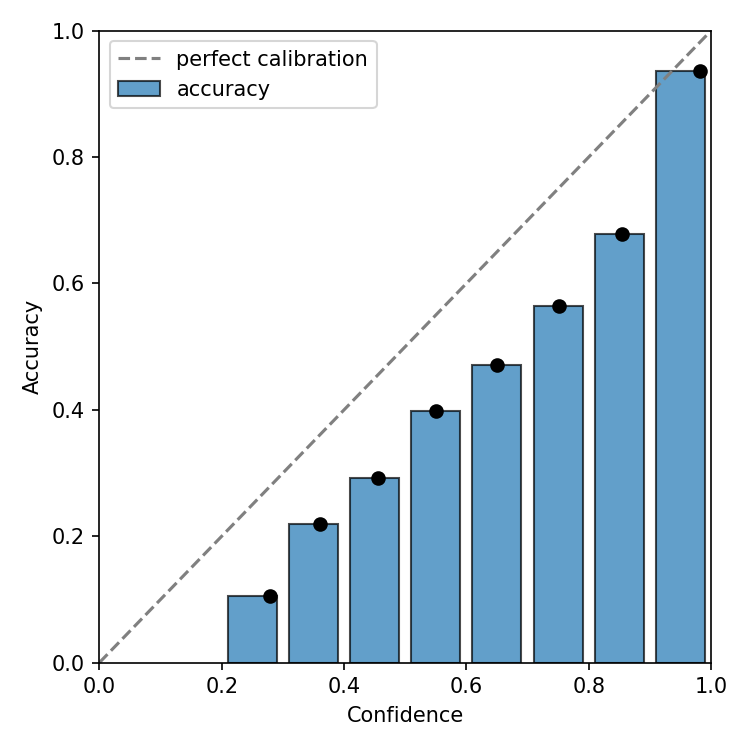
\includegraphics[width=\linewidth]{assets/bracs/tail_reliability_native.png}
    \caption{Severe, native assignment, tail classes}
  \end{subfigure}

  \vspace{0.8em}
  \begin{subfigure}[t]{0.48\linewidth}
    \centering
    
\includegraphics[width=\linewidth]{assets/bracs/tail_reliability_difficulty_aligned.png}
    \caption{Severe, aligned assignment, tail classes}
  \end{subfigure}\hfill
  \begin{subfigure}[t]{0.48\linewidth}
    \centering
    
\includegraphics[width=\linewidth]{assets/bracs/tail_reliability_difficulty_reversed.png}
    \caption{Severe, reversed assignment, tail classes}
  \end{subfigure}
  \caption{BRACS reliability curves for the balanced reference and severe-condition tail classes on the first locked partition.}
  \label{fig:reliability-bracs}
\end{figure}

\begin{figure}[ht]
  \centering
  \begin{subfigure}[t]{0.48\linewidth}
    \centering
    
\includegraphics[width=\linewidth]{assets/tcga_ut/reliability_diagram.png}
    \caption{Balanced reference, all classes}
  \end{subfigure}\hfill
  \begin{subfigure}[t]{0.48\linewidth}
    \centering
    
\includegraphics[width=\linewidth]{assets/tcga_ut/tail_reliability_native.png}
    \caption{Severe, native assignment, tail classes}
  \end{subfigure}

  \vspace{0.8em}
  \begin{subfigure}[t]{0.48\linewidth}
    \centering
    
\includegraphics[width=\linewidth]{assets/tcga_ut/tail_reliability_difficulty_aligned.png}
    \caption{Severe, aligned assignment, tail classes}
  \end{subfigure}\hfill
  \begin{subfigure}[t]{0.48\linewidth}
    \centering
    
\includegraphics[width=\linewidth]{assets/tcga_ut/tail_reliability_difficulty_reversed.png}
    \caption{Severe, reversed assignment, tail classes}
  \end{subfigure}
  \caption{TCGA-UT reliability curves for the balanced reference and severe-condition tail classes on the first locked partition. Both figure sets use ten equal-width confidence bins.}
  \label{fig:reliability-tcga}
\end{figure}



\clearpage
\section{Do Individual Partitions Change the Conclusion?}
\label{app:splits}
Equal-weight pooling is easier to interpret when the individual partitions agree. Tables~\ref{tab:per-split} and~\ref{tab:split-calibration} show every partition-specific deficit on its own endpoint scale; their averages and paired uncertainty are already reported in Appendix~\ref{app:damage-estimates}. The severity checks in Appendix~\ref{app:realized-validity} rule out large allocation-ratio variation as the explanation for these differences.

\begin{table}[H]
\centering\small\setlength{\tabcolsep}{4pt}
% Generated by assets/build_readable_appendix.mjs; do not edit.
\begin{tabular}{@{}lllrrr@{}}
\toprule
Dataset & Comparison & Assignment & Partition 1 & Partition 2 & Partition 3 \\
\midrule
BRACS & Patient shortage & Native & 2.52 & 0.75 & 5.47 \\
BRACS & Patient shortage & Aligned & 2.52 & 0.67 & 5.92 \\
BRACS & Patient shortage & Reversed & 2.00 & 0.47 & 5.39 \\
BRACS & Moderate & Native & 3.67 & 3.53 & 2.83 \\
BRACS & Moderate & Aligned & 1.63 & 2.97 & -0.12 \\
BRACS & Moderate & Reversed & 8.61 & 6.76 & 9.14 \\
BRACS & Severe & Native & 4.67 & 5.99 & 5.69 \\
BRACS & Severe & Aligned & 1.19 & 7.30 & 4.41 \\
BRACS & Severe & Reversed & 12.88 & 12.87 & 13.94 \\
BRACS & Severe spread & Native & 5.63 & 9.98 & 9.68 \\
BRACS & Severe spread & Aligned & 5.56 & 3.84 & 3.04 \\
BRACS & Severe spread & Reversed & 14.29 & 11.60 & 15.40 \\
TCGA-UT & Patient shortage & Native & 4.14 & 4.82 & 5.33 \\
TCGA-UT & Patient shortage & Aligned & 4.35 & 4.69 & 5.45 \\
TCGA-UT & Patient shortage & Reversed & 4.23 & 4.82 & 5.46 \\
TCGA-UT & Moderate & Native & 0.56 & 0.36 & 0.17 \\
TCGA-UT & Moderate & Aligned & 0.08 & 0.13 & 0.19 \\
TCGA-UT & Moderate & Reversed & 0.50 & 0.73 & 0.13 \\
TCGA-UT & Severe & Native & 1.87 & 1.66 & 1.82 \\
TCGA-UT & Severe & Aligned & 1.34 & 1.52 & 1.14 \\
TCGA-UT & Severe & Reversed & 1.40 & 1.60 & 1.35 \\
TCGA-UT & Severe spread & Native & 5.07 & 4.55 & 5.26 \\
TCGA-UT & Severe spread & Aligned & 3.05 & 2.74 & 3.44 \\
TCGA-UT & Severe spread & Reversed & 2.50 & 2.14 & 2.58 \\
\bottomrule
\end{tabular}

\caption{Balanced-accuracy deficit by partition, in percentage points. Positive means damage. Partitions 1--3 correspond to stored partition identifiers 0--2.}
\label{tab:per-split}
\end{table}
\begin{table}[H]
\centering\small\setlength{\tabcolsep}{4pt}
% Generated by assets/build_readable_appendix.mjs; do not edit.
\begin{tabular}{@{}lllrrr@{}}
\toprule
Dataset & Comparison & Assignment & Partition 1 & Partition 2 & Partition 3 \\
\midrule
BRACS & Patient shortage & Native & 0.070 & 0.171 & 0.171 \\
BRACS & Patient shortage & Aligned & 0.070 & 0.148 & 0.202 \\
BRACS & Patient shortage & Reversed & 0.060 & 0.138 & 0.204 \\
BRACS & Moderate & Native & 0.027 & 0.092 & 0.437 \\
BRACS & Moderate & Aligned & 0.598 & 0.243 & 0.298 \\
BRACS & Moderate & Reversed & 0.410 & 0.037 & 1.814 \\
BRACS & Severe & Native & 0.483 & 0.160 & 1.420 \\
BRACS & Severe & Aligned & 0.306 & 0.978 & 0.904 \\
BRACS & Severe & Reversed & 1.266 & 1.567 & 2.398 \\
BRACS & Severe spread & Native & 0.357 & 0.183 & 0.075 \\
BRACS & Severe spread & Aligned & 1.144 & 0.703 & 0.877 \\
BRACS & Severe spread & Reversed & 1.489 & 0.941 & 0.956 \\
TCGA-UT & Patient shortage & Native & 0.209 & 0.356 & 0.224 \\
TCGA-UT & Patient shortage & Aligned & 0.207 & 0.343 & 0.226 \\
TCGA-UT & Patient shortage & Reversed & 0.203 & 0.347 & 0.224 \\
TCGA-UT & Moderate & Native & -0.197 & -0.159 & -0.241 \\
TCGA-UT & Moderate & Aligned & -0.125 & -0.148 & -0.080 \\
TCGA-UT & Moderate & Reversed & -0.069 & -0.057 & -0.060 \\
TCGA-UT & Severe & Native & -0.190 & -0.187 & -0.129 \\
TCGA-UT & Severe & Aligned & 0.133 & 0.177 & 0.119 \\
TCGA-UT & Severe & Reversed & -0.011 & -0.091 & 0.010 \\
TCGA-UT & Severe spread & Native & 0.149 & 0.273 & 0.156 \\
TCGA-UT & Severe spread & Aligned & 0.224 & 0.137 & 0.236 \\
TCGA-UT & Severe spread & Reversed & 0.063 & 0.106 & 0.073 \\
\bottomrule
\end{tabular}

\caption{Tail-group NLL deficit by partition, in nats. Negative values mean improved probability quality. These partition estimates do not replace pooled patient-bootstrap inference.}
\label{tab:split-calibration}
\end{table}

\noindent BRACS balanced-accuracy damage from patient shortage is smallest in partition 2 and largest in partition 3, so two partitions carry most of the pooled magnitude. TCGA-UT repeats the pooled deficit under a stronger patient-coverage contrast. Agreement on the broad mechanism therefore coexists with substantial uncertainty about its magnitude in a particular split.

\section{What Additional Computation Was Required?}
\label{app:cost}
The useful comparison is additional cost against cross-entropy in the same condition. Tables~\ref{tab:cost} and~\ref{tab:cost-tcga} summarize each method's minimum and maximum recorded differences across assignments and conditions. Minutes denote accelerator time; MiB denotes peak memory divided by $2^{20}$. Examples are processed presentations, Unique is the recorded unique-exposure count, and Parameters is model size. These ranges describe measured variation, not uncertainty intervals; rounded zeros can hide small differences.

\begin{table}[H]
\centering\footnotesize\setlength{\tabcolsep}{3pt}
% Generated by assets/build_readable_appendix.mjs; do not edit.
\begin{tabular}{@{}>{\raggedright\arraybackslash}p{3.8cm}rrrrr@{}}
\toprule
Method & Minutes & MiB & Examples & Unique & Parameters \\
\midrule
Balanced sampling & \num{0.0} & \num{-15.9} to \num{0.0} & \num{0} & \num{-4} to \num{0} & \num{0} \\
CE + soft $F_1$ & \num{0.2} to \num{0.8} & \num{-15.9} to \num{0.0} & \num{0} & \num{-4} to \num{0} & \num{0} \\
CE + soft MCC & \num{0.1} & \num{-15.9} to \num{15.9} & \num{0} & \num{-4} to \num{0} & \num{0} \\
CFAL & \num{0.1} to \num{0.2} & \num{1037.6} to \num{1085.3} & \num{0} & \num{0} & \num{-7} \\
Nominal support & \num{0.0} & \num{-15.9} to \num{15.9} & \num{0} & \num{0} & \num{0} \\
cRT & \num{0.1} & \num{-19.3} to \num{-3.3} & \num{129} & \num{0} & \num{0} \\
Focal loss & \num{0.0} to \num{0.1} & \num{-15.9} to \num{15.9} & \num{0} & \num{0} & \num{0} \\
Independent support & \num{0.0} & \num{-0.2} to \num{0.0} & \num{0} & \num{0} & \num{0} \\
Independent support (matched $\beta$) & \num{0.0} & \num{-0.2} to \num{0.0} & \num{0} & \num{0} & \num{0} \\
Logit adjustment (train) & \num{0.0} & \num{-15.9} to \num{0.0} & \num{0} & \num{0} & \num{0} \\
OKO & \num{0.0} to \num{0.1} & \num{-16.5} to \num{31.1} & \num{2727} to \num{2983} & \num{-80} to \num{0} & \num{3591} \\
Difficulty & \num{0.0} & \num{-15.9} to \num{15.9} & \num{0} & \num{0} & \num{0} \\
Logit adjustment (post-hoc) & \num{-0.2} & \num{-3331.2} to \num{-3315.0} & \num{-577400} & \num{-19330} & \num{0} \\
Diversity & \num{0.0} to \num{0.1} & \num{-10.9} to \num{34.1} & \num{0} & \num{0} & \num{0} \\
Prevalence & \num{0.0} & \num{-15.9} to \num{15.9} & \num{0} & \num{0} & \num{0} \\
\bottomrule
\end{tabular}

\caption{BRACS additional cost against matched cross-entropy. Post-hoc adjustment records incremental work after checkpoint reuse; its negative training counts are not end-to-end savings.}
\label{tab:cost}
\end{table}
\begin{table}[H]
\centering\footnotesize\setlength{\tabcolsep}{3pt}
% Generated by assets/build_readable_appendix.mjs; do not edit.
\begin{tabular}{@{}>{\raggedright\arraybackslash}p{3.8cm}rrrrr@{}}
\toprule
Method & Minutes & MiB & Examples & Unique & Parameters \\
\midrule
Balanced sampling & \num{0.0} to \num{0.1} & \num{-15.9} to \num{0.1} & \num{0} & \num{-10} to \num{0} & \num{0} \\
CE + soft $F_1$ & \num{1.7} to \num{3.2} & \num{-15.9} to \num{15.9} & \num{0} & \num{-10} to \num{0} & \num{0} \\
CE + soft MCC & \num{0.1} to \num{0.2} & \num{-15.9} to \num{15.9} & \num{0} & \num{-10} to \num{0} & \num{0} \\
CFAL & \num{0.2} to \num{0.8} & \num{14514.9} to \num{14543.5} & \num{0} & \num{0} & \num{-30} \\
Nominal support & \num{-0.1} to \num{0.1} & \num{-15.9} to \num{15.9} & \num{0} & \num{0} & \num{0} \\
cRT & \num{0.2} to \num{0.5} & \num{-19.3} to \num{12.6} & \num{43} & \num{0} & \num{0} \\
Focal loss & \num{0.0} to \num{0.2} & \num{-15.9} to \num{0.0} & \num{0} & \num{0} & \num{0} \\
Independent support & \num{-0.1} to \num{0.1} & \num{-15.9} to \num{15.9} & \num{0} & \num{0} & \num{0} \\
Independent support (matched $\beta$) & \num{-0.1} to \num{0.1} & \num{-15.9} to \num{0.1} & \num{0} & \num{0} & \num{0} \\
Logit adjustment (train) & \num{-0.2} to \num{0.1} & \num{-15.9} to \num{31.8} & \num{0} & \num{0} & \num{0} \\
OKO & \num{0.2} to \num{0.4} & \num{-16.5} to \num{15.2} & \num{396} to \num{524} & \num{-21} to \num{0} & \num{15390} \\
Difficulty & \num{-0.1} to \num{0.2} & \num{-15.9} to \num{15.9} & \num{0} & \num{0} & \num{0} \\
Logit adjustment (post-hoc) & \num{-0.7} to \num{-0.5} & \num{-18024.4} & \num{-1340000} & \num{-44660} & \num{0} \\
Diversity & \num{0.0} to \num{0.2} & \num{-14.0} to \num{37.8} & \num{0} & \num{0} & \num{0} \\
Prevalence & \num{0.0} to \num{0.1} & \num{-15.9} to \num{0.0} & \num{0} & \num{0} & \num{0} \\
\bottomrule
\end{tabular}

\caption{TCGA-UT additional cost, with the same units and aggregation as Table~\ref{tab:cost}. Exposure differences and memory overhead vary by mechanism.}
\label{tab:cost-tcga}
\end{table}

\noindent Exposure matching removes most differences in data volume, while integral update counts leave residual mismatches for methods such as OKO and two-stage classifier retraining. CFAL has substantially higher peak memory than cross-entropy in both datasets. Post-hoc logit adjustment reuses a trained checkpoint, so its incremental training cost cannot be compared with a complete training run without including that checkpoint's cost. These distinctions are more informative than a single universal ranking of computational expense.
